\chapter{Erstellung des softaware/webdev-\\Docker-Containers}
\label{cha:implementation}
In diesem Abschnitt wird beschrieben, aus welchen Bestandteilen der Container besteht, warum diese Entscheidungen getroffen wurden und welche Probleme und Hürden sich bei der Entwicklung ergaben.
Weiters wird dargestellt, in welchen Aspekten der Container durch neue Kenntnisse beim Einsatz in echten Projekten weiterentwickelt wurde.

\section{Anwendungsszenarien}
\label{sec:usage}
Wie in \cref{cha:concept} erläutert, ist die grundlegende Idee des Containers, Node.js und npm oder yarn als versionierbare Abhängigkeit zu einem Projekt hinzuzufügen.
Anstatt der lokalen Installation dieser Werkzeuge wird lediglich Docker auf dem System benötigt.
Folgend kann der Container, wie in \cref{lst:docker-run-container} dargestellt, gestartet werden.
\begin{lstlisting}[caption=Kommando zum Starten des softaware/webdev-Containers, language=bash, label=lst:docker-run-container]
docker container run -it --rm -v ${pwd}:/usr/src/app softaware/webdev:alpine-8.1.2
\end{lstlisting}
Das Kommando \verb|docker container run| entstammt der neuen Docker-CLI (seit Version 1.13 enthalten) und erzeugt einen Container auf Basis eines Images.
Der Parameter \verb|-it| erzeugt eine interaktive Shell, die mit dem Container verbunden ist.
Durch \verb|--rm| wird der Container nach dem Stoppen wieder entfernt.
Container sollten grundsätzlich keine Daten beinhalten, wodurch diese Option möglich und das System sauber gehalten wird.
Erst durch \verb|-v ${pwd}:/usr/src/app| können die Daten des Containers persistiert werden.
Dieses Kommando bindet das aktuelle Verzeichnis in das Arbeitsverzeichnis des Containers ein.
Dadurch können sowohl der Host als auch der Container gleichzeitig mit diesem Verzeichnis arbeiten, wodurch es möglich wird, dass die Entwicklungsumgebung am Host läuft, npm allerdings im Container.
Am Ende des Kommandos wird das Docker-Image spezifiziert.
In diesem Fall wird die Alpine Linux-Version (vgl. \cref{sec:alpine-vs-debian}) mit der Node.js-Version 8.1.2 verwendet.
Das Ergebnis dieses Kommandos ist in \cref{fig:container-execution} zu sehen.
\begin{figure}[htbp]
    \centering
    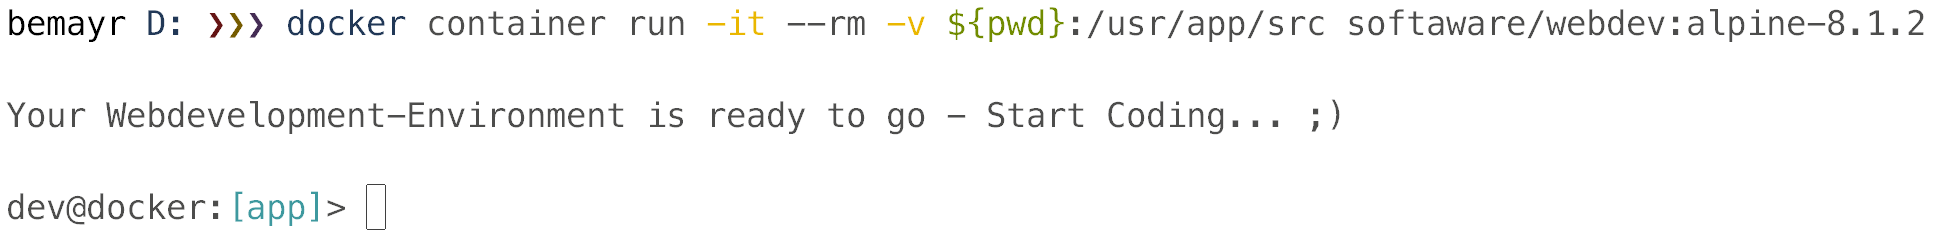
\includegraphics[width=0.95\linewidth,clip]{images/container-execution}
    \caption{Ausgabe beim Start des Containers}
\label{fig:container-execution}
\end{figure}

\subsubsection{Verwendungsmöglichkeiten des Containers}
Für den Container sind grundsätzlich die folgenden drei Anwendungsszenarien vorgesehen:

\begin{enumerate}
    \item Wie im vorangegangenen Beispiel gezeigt, können mithilfe des Containers sehr schnell spezifische Node.js- und npm-Versionen gestartet werden.
        Dies kann \zB zum Initialisieren eines Webprojektes durch \verb|npm init| nützlich sein.
    \item Weiters kann vom softaware/webdev-Image abgeleitet werden, um ein eigenes spezifischeres Image zu erstellen.
        In diesem können \zB weitere Werkzeuge installiert werden oder Ports des Containers explizit freigegeben werden. 
    \item Falls mithilfe der ersten Anwendungsweise ein Projekt erstellt wurde, wird empfohlen, danach das Startkommando mit derselben Containerversion als Skript zum Projekt hinzuzufügen.
        Dadurch kann die Entwicklungsumgebung konsistent reproduziert werden und als Abhängigkeit mit dem Projekt mitversioniert werden.
        Ein Beispiel eines realen Projekts ist in \cref{sec:example} beschrieben.
\end{enumerate}
Im Folgenden wird das \emph{Dockerfile} erläutert, das die Basis des Containers darstellt und die eben beschriebenen Funktionen ermöglicht.

\section{Dockerfile}
\label{sec:dockerfile}
In \cref{lst:dockerfile.alpine} ist der Dockerfile dargestellt, der die Basis des softaware/webdev-Containers bildet.
Dieser wurde vom Autor im Rahmen der Bachelorarbeit erstellt.

\lstinputlisting[caption=Alpine-Dockerfile,label={lst:dockerfile.alpine}]{listings/Dockerfile.alpine}
Im Folgenden werden die einzelnen Kommandos des in \cref{lst:dockerfile.alpine} abgebildeten Dockerfiles Zeile für Zeile erläutert.

\subsubsection{Zeile 2}
Die \verb|FROM|-Anweisung ermöglicht es, dass Docker-Images voneinander erben können.
In diesem Fall wird vom offiziellen Node.js-Image\footnote{\url{https://hub.docker.com/_/node/}} geerbt.
Dieses enthält Node.js, npm und yarn, wodurch die gesamte Basisfunktionalität bereits vorhanden ist.

\verb|{{ node_version }}| ist keine Funktionalität von Docker, dies ist ein Platzhalter für die Versionsnummer des Node.js-Images im Build-Prozess (vgl. \cref{sec:build-process}).
Der Name des offiziellen Node.js-Images beginnt mit der Node.js-Versionsnummer und enthält die Art des Images als Suffix.
In diesem Fall wird vom \emph{alpine}-Image abgeleitet und der Platzhalter im Build-Prozess durch die konkrete Versionsnummer ersetzt.

\subsubsection{Zeile 3}
Die \verb|MAINTAINER|-Anweisung in Dockerfiles wurde ab Version 1.13 durch das flexiblere \verb|LABEL| ersetzt.
Durch den \emph{maintainer} werden Metadaten erstellt, die angeben, wer für dieses Image verantwortlich ist, und an wen sich der Benutzer dessen wenden kann.

\subsubsection{Zeile 6}
Wie im Kommentar in Zeile 5 beschrieben, wird durch die \verb|ENV|-Anweisung die Umgebungsvariable \verb|PATH| erweitert.
Diese Änderung ermöglicht es, lokal installierte Node.js-Anwendungen als Kommandos zu verwenden.

In \cref{sec:global-package-installation} wurde bereits der Unterschied zwischen global und lokal installierten Anwendungen erläutert.
Im Container ist allerdings aufgrund der Isolierung das in \autocite{stackoverflow:nodemodules-hack:online} beschriebene Sicherheitsrisiko wesentlich geringer.
Anstatt der Erstellung eines eigenen Container-Images mit global installierten Paketen sollten diese immer in der \emph{package.json}-Datei erfasst werden.
Dadurch muss kein eigenes Image gewartet werden und auch ohne den Container sind alle Abhängigkeiten des Webprojekts definiert.

Diese Änderung an der Umgebungsvariable ist lediglich aus Kompatibilitätsgründen vorhanden, damit auch ältere Projekte, die sich historisch bedingt auf globale Abhängigkeiten verlassen, im Container verwendet werden können.
Die Konfiguration eines neuen Webprojekts sollte allerdings nach \cref{subsub:packages-best-practice} erfolgen.

\subsubsection{Zeile 9}
Hier wird unter der Verwendung des Alpine Linux-Paketmanagers \emph{apk} die Bourne Again Shell installiert.
Im Gegensatz zur vorinstallierten Almquist Shell ist sie wesentlich weiter verbreitet und bietet mehr Funktionen.
Durch den \verb|--no-cache| Parameter wird die Größe des fertigen Docker-Images möglichst klein gehalten.

\subsubsection{Zeile 12}
In Zeile 12 wird das aktuelle Arbeitsverzeichnis des resultierenden Containers auf \verb|/usr/src/app| gesetzt.
Die \verb|WORKDIR|-Anweisung eines Dockerfiles entspricht im Wesentlichen dem Wechsel in dieses Verzeichnis mit dem Kommando \verb|cd|.

\subsubsection {Zeile 15}
Das Aussehen der Eingabeaufforderung wird in Zeile 15 geändert.
Der Zweck dieser Änderung ist, dass der Entwickler auf den ersten Blick erkennen kann, ob er sich gerade innerhalb des Containers oder außerhalb befindet.

Durch das Dockerfile-Kommando \verb|COPY| wird die Datei \emph{.bashrc} in den Container kopiert.
Diese ist in \cref{lst:.bashrc} abgebildet.
Darin wird in Zeile 2 der Eingabeaufforderung durch das Setzen der Umgebungsvariable \verb|PS1| das Format \emph{dev@docker:[<aktuelles Verzeichnis>]>} zugewiesen.
Die kryptisch aussehende Notation ändert lediglich die Anzeigefarbe des aktuellen Verzeichnisses.
In Zeile 5 wird mit \verb|printf| eine Nachricht beim Start des Containers ausgegeben.
Das Resultat ist in \cref{fig:container-execution} zu sehen.
\lstinputlisting[caption=.bashrc (Bash-Konfigurationsdatei),label={lst:.bashrc},language=bash]{listings/.bashrc}

\subsubsection {Zeile 16}
Beim Ausführen von Skripten, oder beispielsweise dem Deinstallieren von Paketen, bietet npm auf der Kommandozeile die Möglichkeit der Autovervollständigung.
Diese wird aktiviert, indem das Kommando \verb|npm completion| ein Shell-Skript erstellt, das an die benutzerspezifische Shell-Konfiguration angehängt wird.

Das Ergebnis von \verb|npm completion| war in einer früheren Version des Containers bereits in \emph{.bashrc} integriert.
Falls dieses allerdings bei unterschiedlichen npm-Versionen unterschiedlich ausfällt, würde die Autovervollständigung nicht korrekt funktionieren.
Durch das nachträgliche Hinzufügen des Ergebnisses mithilfe der \verb|RUN|-Anweisung ist sichergestellt, dass das Ergebnis von \verb|npm completion| immer zur verwendeten npm-Version passt.

\subsubsection {Zeile 17}
In Zeile 17 wird das Startkommando des Containers auf die Bourne Again Shell festgelegt.
Der verwendete Node.js-Container startet standardmäßig mit dem Kommando \verb|node| ohne weitere Parameter.
Da der softaware/webdev-Container allerdings zur interaktiven Entwicklung gedacht ist, wird dieses Standardverhalten überschrieben.
In \cref{sec:example} wird gezeigt, dass sich dieses Kommando beim Ausführen des Containers überschreiben lässt, wodurch sich der Container auch in Skripte integrieren lässt.

In einer früheren Version des Containers wurde beim Start ein Skript aufgerufen, das überprüft, ob das aktuelle Verzeichnis ein Webprojekt ist.
In diesem Fall wurde \verb|npm install| aufgerufen, um alle Abhängigkeiten zu überprüfen und im Fall von fehlenden Paketen diese nachzuinstallieren.
Da dieses Verhalten für den Benutzer unerwartet ist, allerdings bei jedem Start einige Sekunden kostet, wurde dieses Feature wieder entfernt. 


\section{Build-Prozess}
\label{sec:build-process}
Um ein Docker-Image auf Basis eines Dockerfiles zu erstellen, benötigt es lediglich das Kommando \verb|docker build .|, welches durch den Punkt nach dem Dockerfile im aktuellen Verzeichnis sucht.
Das softaware/webdev-Image ist allerdings im offiziellen Docker Hub\footnote{\url{https://hub.docker.com/}} veröffentlicht, um es ohne weitere Konfiguration mit \verb|docker container run| ausführen zu können.

Anstatt einer Beschreibung zum Erstellen des Images, wurde das in \cref{lst:create-image.ps1} abgebildete Powershell-Skript erstellt.
Mithilfe dessen kann das Image des Containers für existierende Node.js-Versionen automatisch erstellt und veröffentlicht werden.

Docker Hub bietet zwar die Möglichkeit eines automatisierten Builds, wobei das Image bei jeder Änderung automatisch in der Cloud erzeugt wird.
Dieses Service wurde auch evaluiert, Docker Hub benötigt allerdings aufgrund fehlender Funktionen in der GitHub-API Lese- und Schreibrechte auf den gesamten GitHub-Account des verknüpften Repositorys.
Leserechte für das Repository wären kein Problem, da der Quelltext des softaware/webdev-Containers ohnehin öffentlich ist Schreibrechte auf den GitHub-Account der Firma softaware gmbh sind allerdings nicht mit den Unternehmensrichtlinien zu vereinbaren.

\subsubsection{Build-Skript}

Das in \cref{lst:create-image.ps1} abgebildete Build-Skript existiert nicht nur wegen der vorhin beschriebenen Einschränkungen im Docker Hub, sondern auch aufgrund der in \cref{sec:alpine-vs-debian} erläuterten Besonderheiten.
Da der Container Alpine Linux und Debian Linux unterstützt, müssen für jede Node.js-Version zwei Images erstellt werden.
Im Folgenden werden die wichtigsten Funktionen des Build-Skriptes erklärt.
\lstinputlisting[caption=\emph{create-image.ps1} (Build-Skript des Containers),label={lst:create-image.ps1}]{listings/create-image.ps1}

\subsubsection{\texttt{create-image.ps1}}
Das Build-Skript selbst nimmt als einzigen Parameter die Node.js-Version des zu verwendenden Basisimages entgegen.
Zusätzlich können zwei Schalter gesetzt werden:
\begin{enumerate}
    \item \verb|-silent| reduziert die Ausgaben auf ein Minimum.
    \item \verb|-publish| veröffentlicht die erstellten Images auf \url{hub.docker.com}.
        Dazu muss der Verwender in der Docker CLI mit einem Benutzer eingeloggt sein, der Schreibrechte auf das softaware/webdev-Repository im Docker Hub besitzt.
\end{enumerate}

\subsubsection{\texttt{Generate-Images}}
Die Funktion \verb|Generate-Images| ruft für jede registrierte Linux-Distribution die Funktion \verb|Generate-Image| auf.
So können die unterstützten Linux-Distributionen in der Konstante \verb|$DISTRIBUTIONS| zentral erfasst werden.
Dadurch wird die Lesbarkeit des Skripts verbessert
Falls der Container in Zukunft um weitere Distributionen erweitert wird, können diese einfach in das Skript integriert werden.

\subsubsection{\texttt{Generate-Image}}
\verb|Generate-Image| enthält die Logik zum Erstellen der Images.
Auf Basis der Node.js-Version und der Linux-Distribution wird das Image erstellt und, falls gewünscht, danach veröffentlicht:
\begin{itemize}
    \item In Zeile 27 wird das zu verwendende Dockerfile ausgewählt.
    \item Die Zeilen 28 und 29 setzen den Namen des Images, um die Namenskonvention \verb|softaware/webdev:<Linux-Distribution>-<Node.js-Version>| zu erreichen.
    \item In den Zeilen 31 bis 33 wird ein temporäres Dockerfile erstellt, bei dem der Node.js-Versionsplatzhalter (vgl. \cref{sec:dockerfile}) durch eine echte Versionsnummer ersetzt wird.
    \item Auf Basis dieses Dockerfiles wird in Zeile 36 das Image mit dem in Zeile 35 generierten Kommando erstellt.
    \item Schlussendlich wird in Zeile 37 das generierte Dockerfile wieder entfernt.
\end{itemize}
In \cref{fig:create-image} ist eine Beispielausgabe zu sehen, mit der die zwei Images für die Node.js-Version 8.0.0 erstellt und veröffentlicht wurden.
\begin{figure}[htbp]
    \centering
    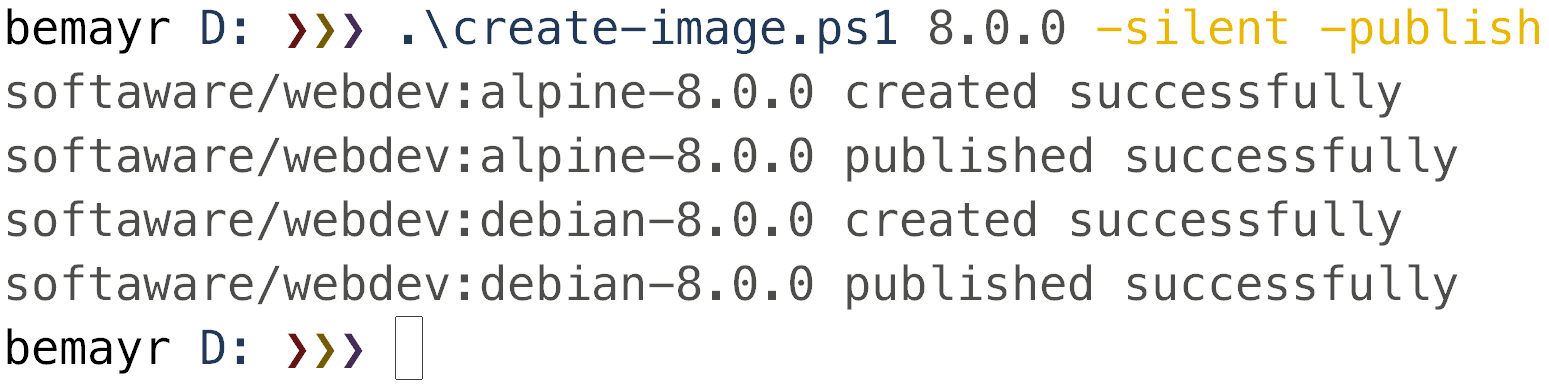
\includegraphics[width=0.75\linewidth,clip]{images/create-image}
    \caption{Ausgabe des Build-Prozesses für Node.js 8.0.0}
\label{fig:create-image}
\end{figure}

\section{Alpine Linux vs. Debian Linux}
\label{sec:alpine-vs-debian}
Um die Imagegröße eines Docker-Containers möglichst gering zu halten, wird der Einsatz der dafür optimierten Linux-Distribution Alpine\footnote{\url{https://alpinelinux.org/}} empfohlen.
Das Alpine-Basisimage hat lediglich eine Größe von fünf Megabyte und ist für die Ausführung im Hauptspeicher optimiert.

Auch vom offiziellen Node.js-Image\footnote{\url{https://hub.docker.com/_/node/}} existiert eine Alpine-Version, die durch die geringe Größe von etwa 17 Megabyte besticht.
In der Dokumentation des Node.js-Containers wird explizit darauf hingewiesen, dass Alpine nicht auf der verbreiteten \verb|glibc|, sondern auf \verb|musl libc| basiert.

Nach ausführlichen Tests wurde festgestellt, dass es bei der Verwendung des Alpine-Containers Probleme mit der Übersetzung von \emph{Sass\footnote{\url{http://sass-lang.com/}}} gibt.
Sass ist eine Sprache, die CSS um die Funktionalität von Variablen und Funktionen erweitert.
Das Problem trat bei der Verwendung des Komponentenframeworks \emph{Kendo UI\footnote{\url{http://www.telerik.com/kendo-ui}}} auf und ist in \autocite{Simko.sass-segfault:online} dokumentiert.
Daher wird nun auch eine auf Debian Linux basierende Version des Containers angeboten, bei der diese Probleme nicht auftreten.

Empfohlen wird aufgrund der wesentlich geringeren Größe (\textasciitilde{}\,20MB anstatt \textasciitilde{}\,250MB) allerdings die Alpine-Version des Containers.

\subsubsection{Debian-Dockerfile}

In \cref{lst:dockerfile.debian} ist der Dockerfile der Debian-Version des Containers dargestellt.

Der Hauptunterschied zum in \cref{lst:dockerfile.alpine} dargestellten Alpine-Image liegt in Zeile 2.
Vom Node.js-Docker-Container existiert sowohl eine Alpine- als auch eine Debian-Version, wobei für Alpine Linux das Präfix \emph{alpine} und für die Debian-Version kein Präfix verwendet wird.
Der zweite Unterschied ist, dass die Bourne Again Shell in Debian Linux bereits inkludiert ist, weshalb diese Installation im Image entfällt.

\lstinputlisting[caption=Debian-Dockerfile,label={lst:dockerfile.debian}]{listings/Dockerfile.debian}

\section{Dokumentation}
\label{sec:documentation}
Dokumentation war neben der möglichst einfachen Benutzung die Hauptaufgabe bei der Erstellung des softaware/webdev-Containers.
Da der Container das erste Open-Source-Projekt der Firma softaware gmbh ist, soll der Fokus auf Dokumentation bei der Verbreitung des Containers helfen, wodurch auch andere Unternehmen davon profitieren können.
Auf folgende Besonderheiten wurde bei der Dokumentation des Projekts Wert gelegt:

\begin{description}
    \item[GitHub] Das gesamte Projekt wurde auf GitHub im Repository softawaregmbh/docker-webdev\footnote{\url{https://github.com/softawaregmbh/docker-webdev}} veröffentlicht.
        Die Dokumentation und der Aufbau der Readme-Datei ist an diejenige des Projekts Cycle.js\footnote{\url{https://github.com/cyclejs/cyclejs}} angelehnt, da diese sehr übersichtlich ist.
    \item[Docker Hub] Wie in \cref{sec:build-process} beschrieben, wurde der fertige Container im Docker Hub veröffentlicht.
        Aufgrund der in jenem Abschnitt beschriebenen Probleme ist die Verknüpfung mit GitHub nicht möglich.
        Diese würde zusätzlich zum automatisierten Build-Prozess den Vorteil bringen, dass die Readme-Datei aus dem GitHub-Repository auch im Docker Hub angezeigt wird.
        Die aktuelle, suboptimale Lösung ist das manuelle Synchronisieren der Readme-Datei von GitHub in den Docker Hub.
    \item[MicroBadger] MicroBadger\footnote{\url{https://microbadger.com/}} ist ein Onlinedienst, der Informationen zu Docker-Images übersichtlich aufbereitet.
        Die Verwendung des Dienstes ist für Open-Source-Projekte kostenlos.
        Zusätzlich werden sogenannte Badges generiert, die in die Dokumentation des Projektes integriert werden können.
        Beim softaware/webdev-Container werden diese verwendet, um die Imagegrößen der Containerversionen übersichtlich darzustellen.
        \cref{fig:microbdager-versions} zeigt diese Übersicht.
\end{description}

\begin{figure}[htbp]
    \centering
    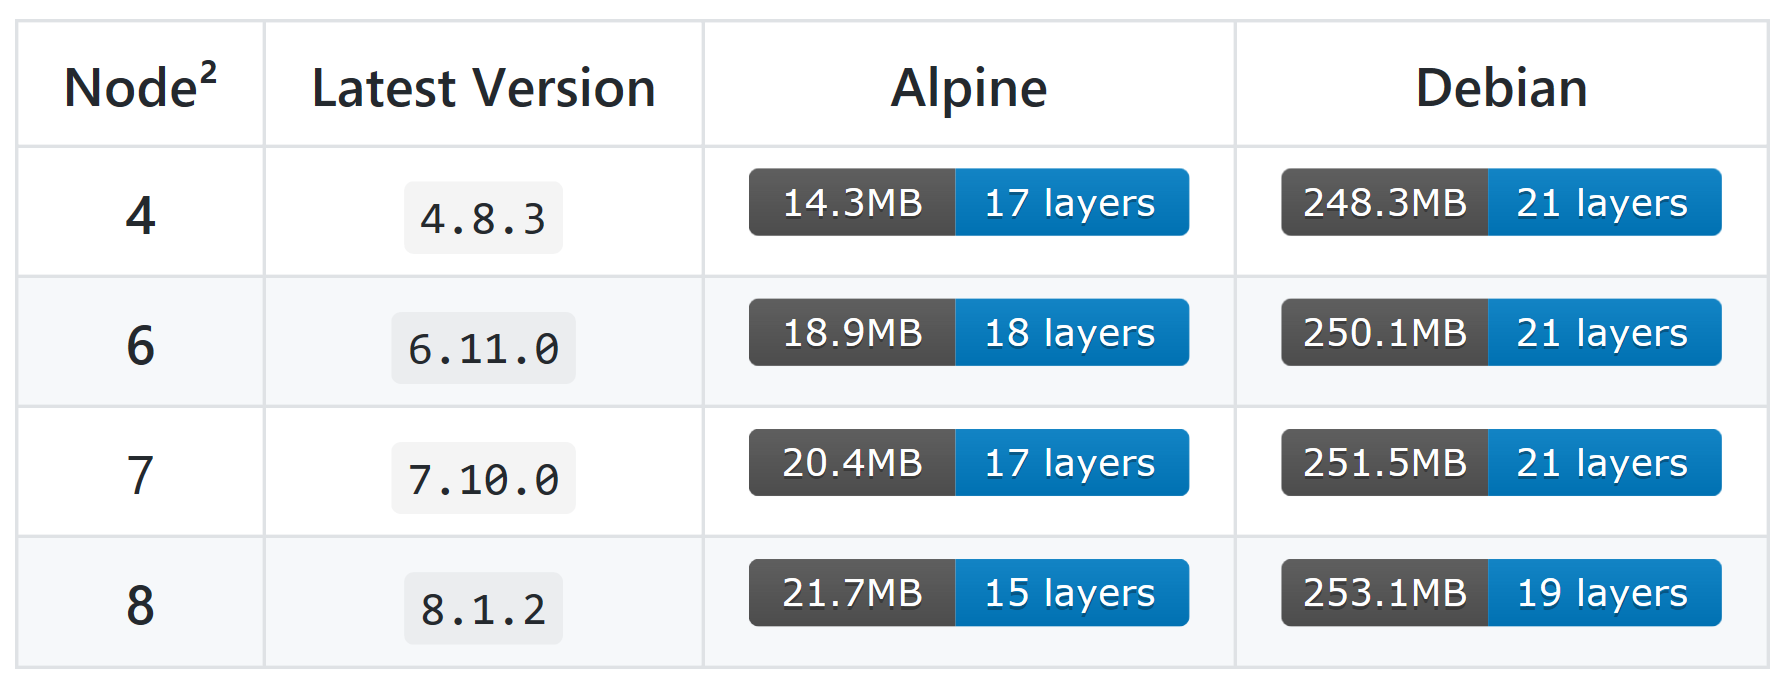
\includegraphics[width=0.75\linewidth,clip]{images/container-versions}
    \caption{MicroBadger-Übersicht über die Container-Versionen}
\label{fig:microbdager-versions}
\end{figure}


\section{Beispiel: Auszug aus einem realen Projekt}
\label{sec:example}
Die in \cref{sec:usage} empfohlene Anwendung des Containers ist die Versionierung durch ein Startskript.
In \cref{lst:docker-webdev.ps1} ist ein solches Powershell-Skript dargestellt, das die Verwendung des Containers vereinfacht.
Der Name dieses Skripts ist in der Firma softaware gmbh normalerweise \emph{docker-webdev.ps1}, wodurch der Entwicklerworkflow über Projektgrenzen hinweg konsistent ist.
Außerdem sind diese Skripte in allen Projekten im Wurzelverzeichnis mitversioniert.

Bei dem Projekt des hier angeführten Skripts handelt es sich um ein Node.js-Webservice, das mit dem Web-Framework \emph{koa\footnote{\url{http://koajs.com/}}} entwickelt wurde. 

\lstinputlisting[caption=docker-webdev.ps1 (Container-Start-Skript),label={lst:docker-webdev.ps1}]{listings/docker-webdev.ps1}
Das Startskript nimmt ein Kommando entgegen, auf Basis dessen ab Zeile 31 entschieden wird, welches Docker-Kommando ausgeführt wird.
Falls kein Kommando spezifiziert wird, wird eine Hilfe, wie in \cref{fig:docker-webdev} dargestellt, ausgegeben.

Der typische Ablauf eines Softwareentwicklers sieht das Starten der Anwendung mit \verb|.\docker-webdev.ps1 start| vor.
Danach können in einer zweiten Powershell-Sitzung mithilfe von \verb|.\docker-webdev.ps1 shell| npm-Kommandos ausgeführt werden.
Dies könnte zum Beispiel die Installation eines Pakets mit \verb|npm install <Paketname>| sein. 
\begin{figure}[htbp]
    \centering
    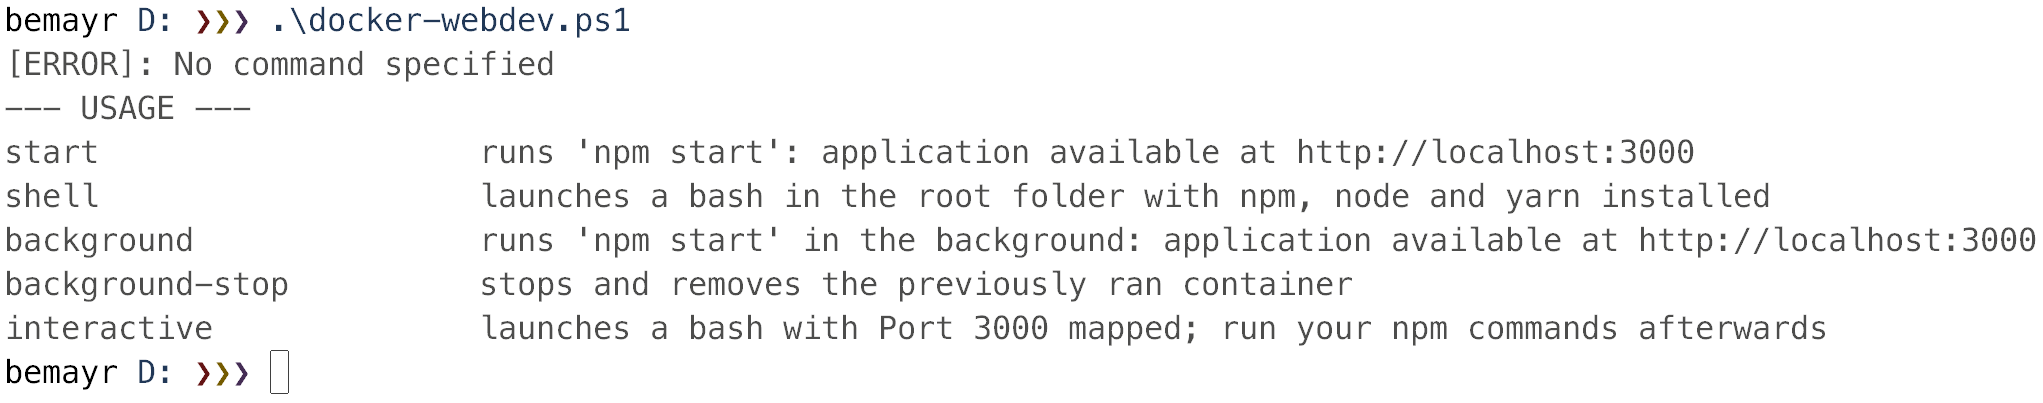
\includegraphics[width=0.95\linewidth,clip]{images/docker-webdev}
    \caption{Hilfe zum Startskript des Containers in einer echten Applikation}
\label{fig:docker-webdev}
\end{figure}


\section{Probleme und Besonderheiten}
\label{sec:container-problems}
Bei der Verwendung des Containers gilt es, folgende Besonderheiten zu beachten:

\begin{itemize}
    \item Wie bereits in \cref{sec:alpine-vs-debian} beschrieben, gibt es bei der Verwendung des Sass-Compilers unter Alpine Linux Probleme.
        Die Lösung dafür ist die Debian-Variante des Containers, bei der diese Probleme nicht auftreten.
    \item Vor der Verwendung des Containers muss das \verb|node_modules|-Verzeichnis gelöscht werden.
        Diese Maßnahme ist notwendig, da es in Node.js native Pakete gibt, bei denen betriebssystemspezifische Varianten installiert werden.
        Nach dem Löschen des Verzeichnisses muss \verb|npm install| im Container ausgeführt werden, damit die richtigen Pakete installiert werden.
    \item Bei der Verwendung des Containers in Kombination mit Entwicklungsumgebungen ist besondere Vorsicht geboten.
        Falls \zB Visual Studio ein Webprojekt erkennt, aktualisiert es im Hintergrund automatisch die npm-Pakete.
        Da dies allerdings außerhalb des Containers geschieht, entstehen Inkonsistenzen im \verb|node_modules|-Verzeichnis.
        Als Lösung wird die Deaktivierung dieser Funktion in der Entwicklungsumgebung vorgeschlagen.
    \item Viele Web-Frameworks werben mit \emph{Hot Reloading}.
        Damit ist die automatische Aktualisierung des Browsers bei Änderungen am Source Code gemeint.
        Bei der Verwendung des Containers muss dazu der Modus konfiguriert werden, der Dateiänderungen erkennt.
        Dieser muss auf Polling umgestellt werden, da es bei Docker ein Problem mit der Erkennung von Änderungen in Dateien gibt, wenn diese zwischen dem Host und dem Container geteilt sind \autocite{Docker.inotify-problem:online}. 
    \item Während der Entwicklung des Containers wurde die Möglichkeit getestet, das \verb|node_modules|-Verzeichnis als eigenes Docker-Volume zu behandeln.
        Dadurch wäre die Performance beim Installieren der Pakete wesentlich besser.
        Allerdings benötigen die Entwicklungsumgebungen Zugriff auf dieses Verzeichnis, um die Autovervollständigung für TypeScript zu ermöglichen, da die Typinformationen direkt aus den Paketen ausgelesen werden.
    \item Die Verwendung des Containers ist optional.
        Falls sich einzelne Entwickler dagegen entscheiden, muss nur sichergestellt sein, dass sie die richtigen Versionen von Node.js und npm installiert haben.
        Dadurch werden heterogene Entwicklungsteams ermöglicht, bei denen nicht jeder Entwickler auf Docker angewiesen ist.
\end{itemize}
